\chapter{Software Design and Development}
\label{chap:software-design}

To implement the 3D MOC solver, the work in this thesis uses the OpenMOC~\ref{openmoc} neutron transport code. This code was developed initial for strictly 2D MOC simulations so great work was required to extend it to 3D MOC calculations. This chapter explains the structure of OpenMOC and the changes that were necessary to increase code flexibility to accommodate 3D MOC calculations. This chapter begins with a general overview of OpenMOC in Section~\ref{sec:openmoc-overview}. The interested reader can find a more complete description of the OpenMOC code in Boyd's thesis~\ref{boyd-ms}. Next, the object oriented design is discussed in greater detail in Section~\ref{sec:object-oriented} with a focus on the changes to accommodate both 2D and 3D simulations. In Section~\ref{sec:user-input} the standard Python user input is discussed as well as the new C++ alternative build which is attractive for high performance computing (HPC) applications where the availability of software required for the Python interface may be limited. Section~\ref{sec:version-control} concludes the chapter with a discussion of development practices and the open source license.

%%%%%%%%%%%%%%%%%%%%%%%%%%%%%%%%%%%%%%%%%%%%%%%%%%%%%%%%%%%%%%%%%%%%%%%%%%%%%%%%
\section{OpenMOC Overview}
\label{sec:openmoc-overview}

OpenMOC is neutron transport code that is written in C++ with a Simplified Wrapper Interface Generator (SWIG)~\cite{swig} to expose the C++ classes and routines to the Python scripting language. In this way, users are able to take advantage of the simplicity and flexibility of the Python language while also having the performance benefits of C++ compiled code. In this way users can work entirely in Python without having to touch the underlying C++ code and also do not have to learn a new input file syntax. This allows for users to write more natural code.

The underlying C++ code of OpenMOC also leverages the use of OpenMP~\cite{openmp} for shared memory parallelism. With the emergence of the 3D solver, distributed parallelism has also been implemented with MPI in the form of domain decomposition, discussed in Chapter~\ref{chap:domain-decomposition}. With this hybrid parallelism design, OpenMOC is able to scale to both many CPU cores and many nodes. 

OpenMOC is built on the use of constructive solid geometry (CSG), which allow complex geometries to be built out of boolean operations -- such as intersections and unions -- of simple surfaces and building blocks termed primitives. In addition, a hierarchy is used to agglomerate collections of primitives together. This approach is particularly useful for reactor geometries which are often highly structured. For example, a typical reactor core is built out of simple \textit{fuel pins}, grouped together into \textit{assemblies}. Assemblies are then grouped together to form the reactor core. An example of a CSG construction of a single assembly is given in Figure~\ref{fig:core-csg}.

\begin{figure}[h!]
	\centering
	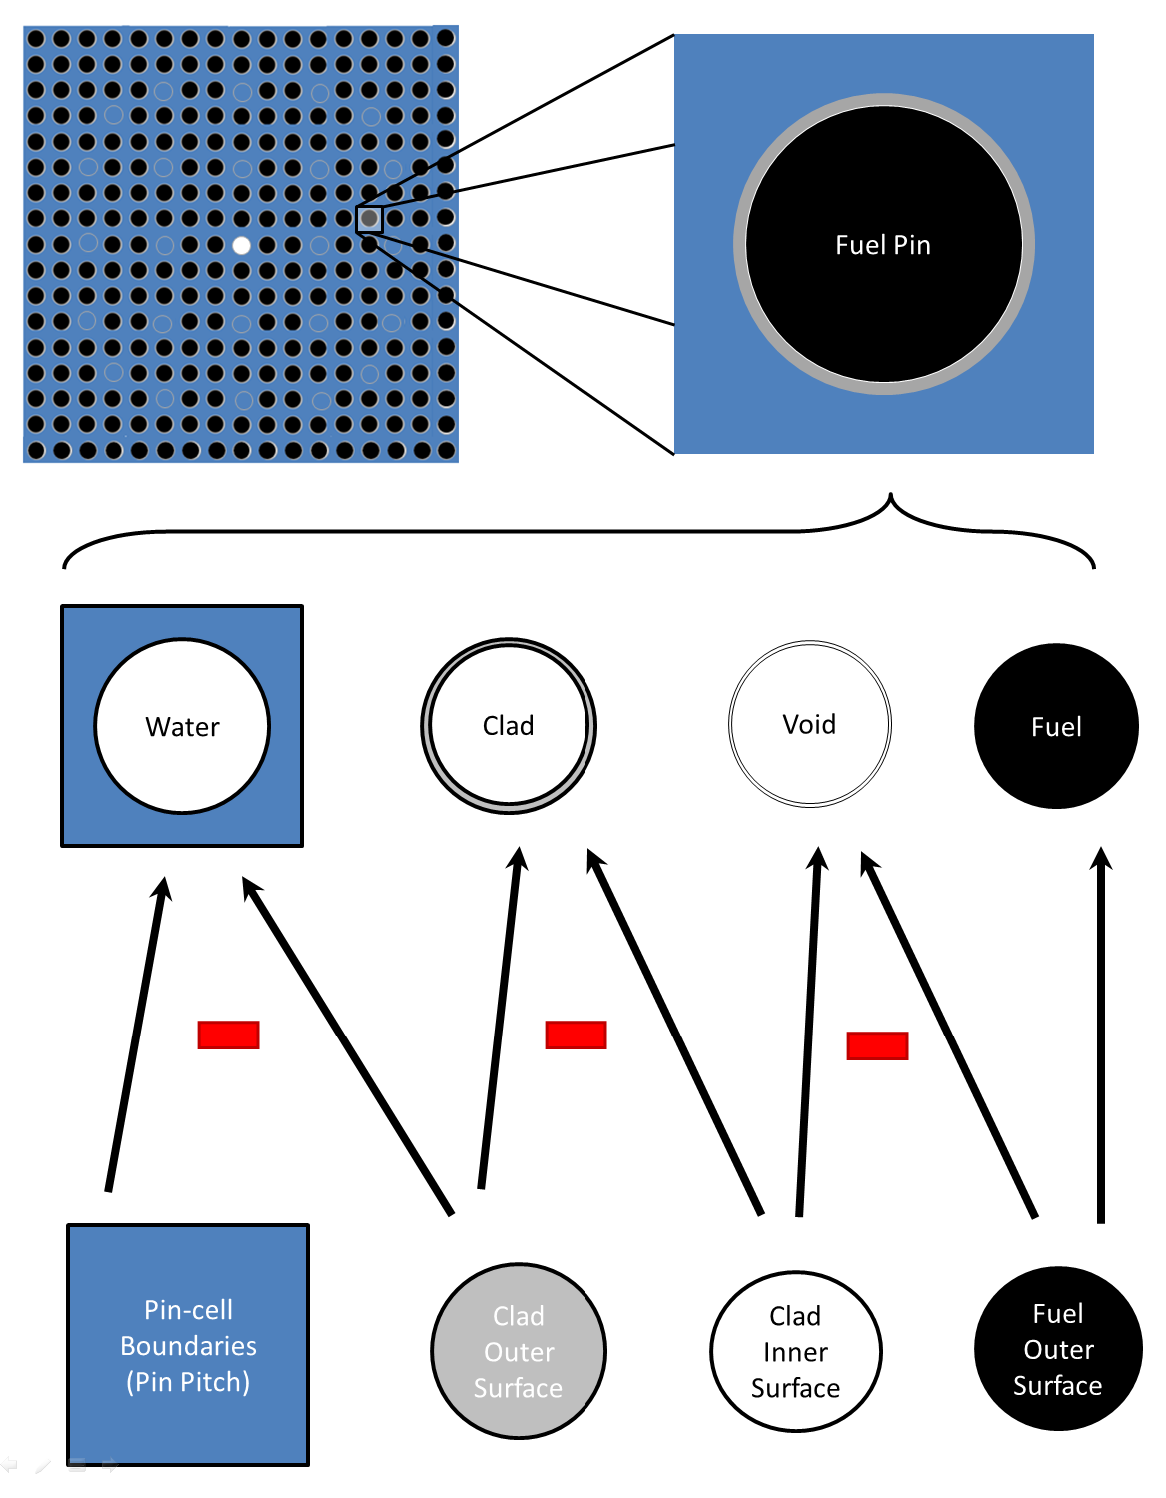
\includegraphics[width=0.9\linewidth]{figures/assembly-csg.PNG}
	\caption[]{The hierarchical CSG construction of a typical assembly.}
	\label{fig:core-csg}
\end{figure}

One of the benefits of the CSG approach is a reduced memory requirements of storing the geometry. Instead of explicitly storing information of each fuel pin within the reactor core, only unique fuel pin types need to be stored. They are then referenced in their parent object. For instance, an assembly contains an lattice of fuel pins. It would contain a mapping of location within the lattice to the unique assembly type, rather than the full information of each fuel pin.

In addition, the formation of a CSG allows ray tracing to be conducted in a general framework, agnostic of the individual primatives. Each \textit{cell} in OpenMOC is comprised of \textit{surface} objects and the half-space of each surface. A half-space determines on which side of the surface the cell is located. Ray tracing fundamentally involves calculating the distance to intersection along a direction. With the CSG framework, each of the bounding surfaces is queried for the distance to intersection. This naturally speeds up ray tracing by not having to check each instance of a surface within the geometry, but rather only the local surfaces. 

Once the geometry is built, OpenMOC generates tracks across the constructed geometry, and solves the neutron transport equation iteratively, as described in Chapter~\ref{chap:moc}. CMFD acceleration can also be included by the user, which employs the underlying methods that were described in Chapter~\ref{chap:cmfd-acceleration}.

Once the neutron transport equation is solved, the solver can be queried to return the scalar flux distribution. In order to visualize the data, OpenMOC includes Python plotting routines for scalar flux data, computed reaction rates, as well as geometric detail and visual diagnostics. 


%%%%%%%%%%%%%%%%%%%%%%%%%%%%%%%%%%%%%%%%%%%%%%%%%%%%%%%%%%%%%%%%%%%%%%%%%%%%%%%%
\section{Object Oriented Design}
\label{sec:object-oriented}

OpenMOC uses the object oriented programming paradigm whereby data structures called \textit{classes} are created that encapsulate both the data and associated subroutines. Object oriented programming generally leads to more resilient code since only the class itself can access its private attributes. An instantiation of a class is termed an \textit{object}. OpenMOC applies many of the principles of object oriented programming including information hiding, inheritance, and polymorphism.

An OpenMOC simulation requires three main components: a geometry, a track generator, and a solver. All of these are C++ classes in OpenMOC and exposed to the user. The user first describes the surfaces, cells, universes, and materials which constitute the geometry in a hierarchical CSG arrangement. The user then instantiates a \texttt{Geometry} object and provides it the root cell of the CSG. Next, a \texttt{TrackGenerator} is instantiated which is provided the \texttt{Geometry} object as well as track generation parameters such as radial ray spacing and number of azimuthal angles. Lastly, a \texttt{Solver} object is instantiated and given the \texttt{TrackGenerator} object along with solver criteria such as the tolerance. The solver can then be called to solve the MOC equations, such as the MOC neutron transport eigenvalue problem.

Extending the OpenMOC solver to 3D simulations required restructuring all of these classes in order to make them more flexible. The goal in extending to 3D simulations was to still maintain the ability to run 2D simulations, if desired. Additionally, to make the code more resilient and simpler, common code reuse should be maximized. Many of the routines present in the 2D simulations would also be used in the 3D simulations so both should use the same code without re-writing those entire sections. Also, users might be interested in running both 2D and 3D simulations on the same problem. Therefore, the input structure should not change much between 2D and 3D simulations. These points illustrate that the code should aim for maximum cohesion between the 2D and 3D modes. This is accomplished by expanding the 2D classes to be more general.

\subsection{\texttt{Geometry} Class Updates}
\label{sec:oo-geometry}

The \texttt{Geometry} class is altered to accommodate piecewise \textit{extruded geometries}. Extruded geometries are configurations in which the geometry looks the same at every axial level. A piecewise extruded geometry is a geometry that can be formed as the union of a finite number of extruded geometries. For instance, a fuel rod with end caps would fit the description of an extruded geometry but a sphere would not. Most practical reactor applications are indeed piecewise extruded geometries so this is not a very strong limitation. 

With the change from 2D geometries to piecewise axially extruded geometries, circles are transformed to $z$-cylinders (cylinders with the major axis vertical) and $z$-planes are added with a similar structure to the $x$ and $y$ planes already incorporated in OpenMOC. With this new geometry paradigm, 2D problems are thought of as simulating an $xy$ slice of a 3D geometry at a given $z$ height. By default this height is assumed to be 0.0 in order to limit the complexity of user input for 2D simulations.

\subsection{\texttt{TrackGenerator} Class Updates}
\label{sec:oo-trackgenerator}

Since tracks are built on a 2D projection, the 3D track generator must have all the functionality of the regular 2D track generator.

\subsection{\texttt{Solver} Class Updates}
\label{sec:oo-solver}

Solver - CPUSolver

%%%%%%%%%%%%%%%%%%%%%%%%%%%%%%%%%%%%%%%%%%%%%%%%%%%%%%%%%%%%%%%%%%%%%%%%%%%%%%%%
\section{Modular Structure}
\label{sec:modular-structure}

code reuse

For example, MOC can largely be described as an algorithm that performs a ray trace then computes equations over the segments formed from the ray trace. Many different ray tracing algorithms could be used with the underlying equations and solver remaining theoretically unchanged. However, if the code is rigid, each new ray tracing algorithm would require an entire code re-write. 

Talk about ray tracer comparison as a possibility

%%%%%%%%%%%%%%%%%%%%%%%%%%%%%%%%%%%%%%%%%%%%%%%%%%%%%%%%%%%%%%%%%%%%%%%%%%%%%%%%
\section{User Input}
\label{sec:user-input}

In terms of input structure, the 3D MOC updates to OpenMOC were structured to minimize the amount of work required to convert a 2D input to a 3D input. From a fully defined 3D geometry, including $z$-planes, the only difference in input between a 2D and 3D simulation is the definition of the track generator. A regular 2D \texttt{TrackGenerator} object supplied to a solver will trigger the 2D MOC solver, whereas a \texttt{TrackGenerator3D} object will trigger the 3D MOC solver.

If the Geometry was written in two dimensions without specifying $z$-planes, the geometry will need to be bounded in order to have a well defined 3D MOC problem. In theory, a 2D simulation implies infinite dimensions axially so if a bounded 3D geometry is provided to a regular 2D \texttt{TrackGenerator} object, a warning will be triggered, but the simulation will still run assuming infinite axial dimensions.

To facilitate running on systems which do not have thorough Python support or have difficulty transferring MPI communicator objects between Python and C++ for domain decomposed simulations, an alternative C++ build was implemented. This build uses a standard C++ Makefile and includes sample inputs in C++.

%%%%%%%%%%%%%%%%%%%%%%%%%%%%%%%%%%%%%%%%%%%%%%%%%%%%%%%%%%%%%%%%%%%%%%%%%%%%%%%%%
\section{Version Control and Licensing}
\label{sec:version-control}

OpenMOC utilizes Git version control and an open source distribution is hosted on GitHub at \url{https://github.com/mit-crpg/OpenMOC.git}. Git is a free and open source version control distribution that is becoming the software industry standard for version control. GitHub uses the Git distribution to host software distributions, both open source and closed source. Pull requests to the \textit{develop} branch form the basis by which the code evolves. Anyone in the public can contribute to the code by making a pull request to the develop branch. 

The OpenMOC code has been approved for open source release by the MIT Technology Licensing Office (TLO) under the MIT/X license. This license allows anyone to download the software without restriction. In addition, modifications to the software may be published, distributed, or sold. OpenMOC is designed with the intent of experimenting with new ideas within MOC simulations. This is further aided by the new flexible structure detailed in this chapter. The goal of OpenMOC is to promote an active reactor physics community where transparent research is possible and new ideas encourage the improvement of nuclear reactor modeling and simulation.